%% 
%% Copyright 2019-2024 Elsevier Ltd
%% 
%% This file is part of the 'CAS Bundle'.
%% --------------------------------------
%% 
%% It may be distributed under the conditions of the LaTeX Project Public
%% License, either version 1.3c of this license or (at your option) any
%% later version.  The latest version of this license is in
%%    http://www.latex-project.org/lppl.txt
%% and version 1.3c or later is part of all distributions of LaTeX
%% version 1999/12/01 or later.
%% 
%% The list of all files belonging to the 'CAS Bundle' is
%% given in the file `manifest.txt'.
%% 
%% Template article for cas-sc documentclass for 
%% double column output.

\documentclass[a4paper,fleqn]{cas-sc}

% If the frontmatter runs over more than one page
% use the longmktitle option.

%\documentclass[a4paper,fleqn,longmktitle]{cas-sc}

\usepackage[numbers,sort&compress]{natbib}

% In-draft instructions for displays awaiting case-level evaluation data.
\definecolor{guideblue}{HTML}{35678F}
\newlength{\displayguidewidth}
\newcommand{\displayguide}[5]{%
  \begingroup
  \setlength{\displayguidewidth}{#1}%
  \setlength{\fboxrule}{0.7pt}%
  \setlength{\fboxsep}{6pt}%
  \noindent\fcolorbox{guideblue}{guideblue!6!white}{%
    \begin{minipage}{\dimexpr\displayguidewidth-2\fboxsep-2\fboxrule\relax}
      \hypersetup{linkcolor=black}%
      \raggedright\small
      {\color{guideblue}\bfseries #2\par}\smallskip
      \textbf{Data needed}\enspace #3\par
      \textbf{Preparation}\enspace #4\par
      \textbf{Acceptance check}\enspace #5\par
    \end{minipage}}%
  \endgroup\par\medskip}
\newcommand{\figureguide}{\displayguide{\dimexpr.88\linewidth+2\fboxsep+2\fboxrule\relax}}

% Use the body-text family for CAS captions, table text, and URLs.
\renewcommand{\sfdefault}{\rmdefault}
\urlstyle{same}

%%%Author macros
\def\tsc#1{\csdef{#1}{\textsc{\lowercase{#1}}\xspace}}
\tsc{WGM}
\tsc{QE}
%%%

% Uncomment and use as if needed
%\newtheorem{theorem}{Theorem}
%\newtheorem{lemma}[theorem]{Lemma}
%\newdefinition{rmk}{Remark}
%\newproof{pf}{Proof}
%\newproof{pot}{Proof of Theorem \ref{thm}}

\begin{document}
\let\WriteBookmarks\relax
\def\floatpagepagefraction{1}
\def\textpagefraction{.001}

% Short title
\shorttitle{}    

% Short author
\shortauthors{}  

% Main title of the paper
\title [mode = title]{Adapting OmniArch for similarity-based extrapolation of airfoil flow fields and turbine blade temperatures}

% Title footnote mark
% eg: \tnotemark[1]
\tnotemark[1] 

% Title footnote 1.
% eg: \tnotetext[1]{Title footnote text}
\tnotetext[1]{} 

% First author
%
% Options: Use if required
% eg: \author[1,3]{Author Name}[type=editor,
%       style=chinese,
%       auid=000,
%       bioid=1,
%       prefix=Sir,
%       orcid=0000-0000-0000-0000,
%       facebook=<facebook id>,
%       twitter=<twitter id>,
%       linkedin=<linkedin id>,
%       gplus=<gplus id>]

\author[1]{}%[<options>]

% Corresponding author indication
\cormark[1]

% Footnote of the first author
\fnmark[1]

% Email id of the first author
\ead{}

% URL of the first author
\ead[url]{}

% Credit authorship
% eg: \credit{Conceptualization of this study, Methodology, Software}
\credit{}

% Address/affiliation
\affiliation[1]{organization={},
            addressline={}, 
            city={},
%          citysep={}, % Uncomment if no comma needed between city and postcode
            postcode={}, 
            state={},
            country={}}

\author[2]{}%[]

% Footnote of the second author
\fnmark[2]

% Email id of the second author
\ead{}

% URL of the second author
\ead[url]{}

% Credit authorship
\credit{}

% Address/affiliation
\affiliation[2]{organization={},
            addressline={}, 
            city={},
%          citysep={}, % Uncomment if no comma needed between city and postcode
            postcode={}, 
            state={},
            country={}}

% Corresponding author text
\cortext[1]{Corresponding author}

% Footnote text
\fntext[1]{}

% For a title note without a number/mark
%\nonumnote{}

% Here goes the abstract
\begin{abstract}
Computational fluid dynamics underpins the design of aircraft and engines, where every
candidate design must be evaluated across many operating conditions. Such workloads require
surrogate models that are both fast and extrapolable, accurate at conditions beyond the
training range. However, current methods trade one for the other. Numerical solvers compute
each condition from the governing equations, but each run takes minutes to hours, and at
extreme conditions the solution may fail to converge or lose accuracy. Neural operators, in
contrast, predict in milliseconds but degrade once the Reynolds number or temperature leaves
the training range. Dimensional analysis has long reduced such problems to a few similarity
variables, but typically for scalar quantities rather than full fields on unstructured
meshes. In this work, we introduce similarity specialization, which rewrites the inputs and
outputs of a pretrained PDE foundation model in the similarity variables of the governing
equations. As in wind-tunnel testing, where similarity parameters carry scale-model
measurements to full-scale flight, these variables carry what is learned at training
conditions to new ones, and the model learns only the scale effects that the similarity law
leaves out. In similarity variables, extrapolation in physical parameters largely reduces to
interpolation. We present OmniArch-Aero, which tokenizes unstructured meshes into spatial
blocks, reads them with the pretrained OmniArch backbone, and decodes fields at arbitrary
points through cross-attention. On Reynolds-number extrapolation in AirfRANS, OmniArch-Aero
lowers the lift-coefficient error by 91\% relative to the best published model and predicts
each flow field in 0.22 s, compared with about 25 min for the RANS solver. These results
suggest a principle for physics-aware foundation models: learn in similarity variables, not
in physical units.
\end{abstract}

% Place the graphical abstract in the first-page title block.
\BeforeBeginEnvironment{Abstract}{%
  \par
  \begingroup
  \vspace{5pt}%
  \noindent G\,R\,A\,P\,H\,I\,C\,A\,L\quad A\,B\,S\,T\,R\,A\,C\,T\par
  \dashrule[.2pt]{2pt}{5pt}%
  \noindent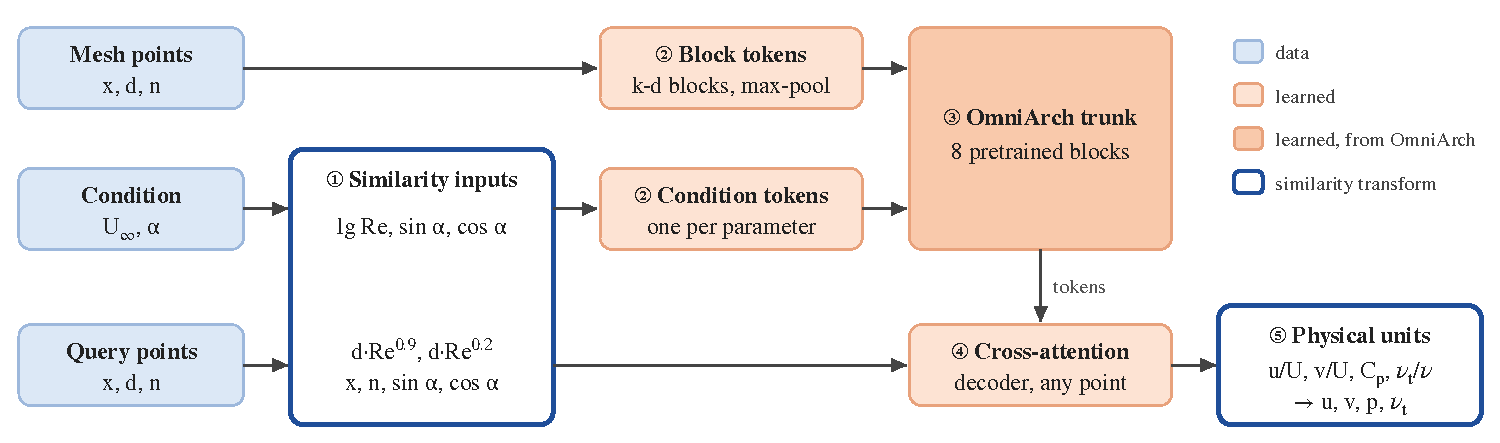
\includegraphics[width=.5\linewidth]{figs/overview.pdf}\par
  \dashrule{5pt}{10pt}%
  \endgroup
}

% Keywords
% Each keyword is seperated by \sep
\begin{keywords}
Dimensional analysis \sep
PDE foundation models \sep
Unstructured meshes \sep
Parameter extrapolation \sep
Airfoil aerodynamics \sep
Turbine blade cooling
\end{keywords}

\maketitle

% Main text
\section{Introduction}\label{sec:introduction}
\noindent{\small\textbf{Page budget:} approx.\ 2 pages\quad \textbf{Status:} Draft ready for review}\par

A single aerodynamic or thermal design is evaluated at multiple operating conditions.
For an airfoil, the near-wall flow and surface pressure determine the aerodynamic loads
used to assess performance. For a cooled turbine blade, the metal temperature field
locates hot regions and informs the assessment of thermal margins~\citep{Han2013}. A new operating
condition typically requires another solution of the governing equations, including
the coupled fluid and solid problem for the blade. A surrogate can reduce this cost
by reusing information from available solutions~\citep{Brunton2020,Benner2015}. Its use at an operating condition
outside the sampled range depends on whether it can recover the field and the
engineering quantities derived from it.

Neural operators such as the Fourier neural operator (FNO) and DeepONet learn mappings
between functions, allowing a trained model to approximate a family of solutions to
parametric partial differential equations~\citep{Li2021FNO,Lu2021DeepONet}. Geometry-aware methods such as Transolver
extend operator learning to complex geometries~\citep{Wu2024Transolver}. Scientific foundation models such
as OmniArch provide pretrained parameters that can initialise models for downstream
tasks~\citep{Chen2025OmniArch}. These developments make full-field surrogates feasible on irregular domains.
For the tasks considered here, the key question is how well such a surrogate predicts
when the supplied geometry and operating conditions include a Reynolds number or inlet
temperature beyond the training range.

Dimensional analysis supplies a way to distinguish changes in physical scale from
changes in the structure of the solution. The Buckingham \(\Pi\) theorem describes
how dimensional variables can be grouped into dimensionless combinations~\citep{Buckingham1914}.
Bakarji et al.\ used data to identify such groups~\citep{Bakarji2022}.
Oppenheimer et al.\ used dimensionless variables in learning across physical
scales~\citep{Oppenheimer2023}. These studies
motivate using characteristic scales to represent both the operating conditions
and the predicted fields. For a pretrained surrogate on an unstructured mesh, the
relevant choice is which scales to account for explicitly and which variations to
learn from the available reference solutions.

The two applications call for different choices of similarity variables. In airfoil
flow, the freestream speed \(U_\infty\) sets the scales of velocity and kinematic
pressure through \(U_\infty\) and \(U_\infty^2\), respectively. The Reynolds number
still affects the dimensionless momentum balance, so the network must represent its
effect on the scaled flow. For the blade, the difference between mainstream and
coolant inlet total temperatures provides a scale for the metal temperature field.
Similarity scaling for cooled turbine metal temperatures has been studied theoretically
and in experiments on nozzle guide vanes~\citep{Luque2016,Luque2017}. Studies of overall
cooling effectiveness also show a dependence on the inlet temperature ratio and gas
properties~\citep{Cartlidge2024}. On a fixed blade mesh,
lower-temperature solutions can be used to estimate how that dimensionless field
changes at corresponding nodes.

We develop OmniArch-Aero to incorporate these task-specific representations into
field prediction on unstructured meshes. The network encodes the mesh as spatial
blocks, processes their tokens with a backbone initialised from pretrained OmniArch
parameters, and decodes the field at query points. For the airfoil task, similarity
transformations define the operating inputs and the predicted flow variables. For
the cooled blade, a nodewise prior fitted to lower-temperature solutions provides
the initial dimensionless temperature field, and the network learns a residual
correction. The two tasks use the same architecture and are trained separately.
The problem definitions and the transformations are given in
Sections~\ref{sec:problem-statement} and~\ref{sec:methodology}, respectively.

The study on the AirfRANS benchmark~\citep{Bonnet2022AirfRANS} (Section~\ref{sec:airfrans-results}) compares the dimensional and
similarity configurations at Reynolds numbers outside the training interval and
evaluates the lift recovered from the predicted fields. The blade study
(Section~\ref{sec:blade-results}) holds the geometry and mesh fixed and compares
direct similarity conversion, a nodewise temperature prior, and the prior with
a learned correction. This comparison separates the contribution of the
low-temperature prior from the additional improvement obtained by learning the
residual at the two high-temperature test conditions.

% Numbered list
% Use the style of numbering in square brackets.
% If nothing is used, default style will be taken.
%\begin{enumerate}[a)]
%\item 
%\item 
%\item 
%\end{enumerate}  

% Unnumbered list
%\begin{itemize}
%\item 
%\item 
%\item 
%\end{itemize}  

% Description list
%\begin{description}
%\item[]
%\item[] 
%\item[] 
%\end{description}  

% Example float syntax is available in cas-sc-sample/cas-sc-sample.tex.

% Uncomment and use as the case may be
%\begin{theorem} 
%\end{theorem}

% Uncomment and use as the case may be
%\begin{lemma} 
%\end{lemma}

%% The Appendices part is started with the command \appendix;
%% appendix sections are then done as normal sections
%% \appendix

\section{Problem statement}\label{sec:problem-statement}
\noindent{\small\textbf{Page budget:} approx.\ 2 pages\quad \textbf{Status:} Draft ready for review}\par

We study Reynolds-number extrapolation across a range of airfoils and predict
the temperature field of a cooled turbine blade of fixed geometry at mainstream
inlet total temperatures beyond the training range.

\subsection{Airfoil flow and Reynolds-number extrapolation}\label{subsec:airfoil-problem}
\noindent{\small\textbf{Page budget:} approx.\ 1 page}\par

We consider steady, two-dimensional, incompressible flow past an airfoil of chord $L$
at freestream speed $U_\infty$ and angle of attack $\alpha$. AirfRANS provides the
reference Reynolds-averaged Navier--Stokes (RANS) fields. For constant density $\rho$
and kinematic viscosity $\nu$ and negligible body forces, scaling by $L$ and $U_\infty$
gives the dimensionless continuity and momentum equations~\citep{Pope2000}
\begin{equation}
  \label{eq:airfoil-rans}
  \begin{aligned}[b]
    &\nabla^*\!\cdot\mathbf{u}^* = 0, \\
    &(\mathbf{u}^*\!\cdot\nabla^*)\mathbf{u}^*
      = -\nabla^*p^*
        + \frac{1}{Re}\nabla^{*2}\mathbf{u}^*
        - \nabla^*\!\cdot\mathbf{R}^*,
        \qquad Re=\frac{U_\infty L}{\nu}.
  \end{aligned}
\end{equation}
Here $\nabla^*$ denotes differentiation with respect to $\mathbf{x}^*=\mathbf{x}/L$, and
$\mathbf{u}^*=\overline{\mathbf{u}}/U_\infty$. The dimensionless pressure and Reynolds
stress are $p^*=(\overline{p}-p_{\mathrm{ref}})/(\rho U_\infty^2)$ and
$\mathbf{R}^*=\overline{\mathbf{u}'\otimes\mathbf{u}'}/U_\infty^2$, where
$p_{\mathrm{ref}}$ is the reference pressure and $\mathbf{u}'$ is the velocity fluctuation.
In Eq.~\eqref{eq:airfoil-rans}, $1/Re$ weights the molecular viscous term, so the
dimensionless flow can vary with $Re$. AirfRANS uses the $k\!-\!\omega$ SST
turbulence closure and a no-slip condition on the airfoil surface~\citep{Bonnet2022AirfRANS}.

Given the unstructured mesh and freestream conditions, the model predicts the nodal
fields $(u,v,p_{\mathrm{kin}},\nu_t)$. Here $u$ and $v$ are the mean velocity components,
$p_{\mathrm{kin}}$ is the mean pressure divided by density using the dataset's pressure
convention, and $\nu_t$ is the turbulent kinematic viscosity. These fields provide the
training targets (Sections~\ref{subsec:airfoil-similarity} and~\ref{subsec:mesh-to-field}).
We compute the lift coefficient $C_L$ from the wall pressure and viscous shear, using
the same procedure for the predicted and reference fields.

Training uses cases with $Re\in[3\times 10^6,\,5\times 10^6]$. Tests cover both sides
of this interval, with the geometry and angle of attack supplied for each case.
Sections~\ref{subsec:airfrans-setup} and~\ref{subsec:airfrans-errors} describe the split
and evaluate lift prediction accuracy, respectively.

\subsection{Cooled turbine blade and the temperature extrapolation task}\label{subsec:blade-problem}
\noindent{\small\textbf{Page budget:} approx.\ 1 page}\par

The engineering case is a cooled turbine rotor blade with solid domain
$\Omega_{\mathrm{s}}$. Solid conduction and heat transfer at the mainstream and coolant
interfaces govern the metal temperature. Given the mesh and operating conditions,
we predict $T(\mathbf{x})$ at the solid nodes using CFX conjugate heat transfer solutions
as reference. The reference cases record inlet total temperatures, mass flow rates,
outlet static pressure, and rotational speed.

Let $T_g$ and $T_c$ denote the mainstream and coolant inlet total temperatures in the
stationary frame. Scaling by their difference gives the dimensionless temperature
$\theta(\mathbf{x})$ and the corresponding recovery of $T(\mathbf{x})$
\begin{equation}
  \label{eq:blade-temperature-similarity}
  \theta(\mathbf{x})=\frac{T_g-T(\mathbf{x})}{T_g-T_c},
  \qquad
  T(\mathbf{x})=T_g-(T_g-T_c)\,\theta(\mathbf{x}).
\end{equation}
The direct similarity baseline (Section~\ref{subsec:blade-setup}) retains the low-temperature
reference field $\theta_{\mathrm{ref}}(\mathbf{x})$ and applies
Eq.~\eqref{eq:blade-temperature-similarity} with the target $T_g$ and $T_c$.
Temperature-dependent properties can alter solid conduction and interfacial heat transfer.
The temperature prior (Section~\ref{subsec:blade-prior}) models how $\theta$ varies
across operating conditions.

The common blade geometry and mesh allow nodewise comparisons of $\theta$ across cases.
The five similarity parameters supplied to the network are the coolant-to-mainstream mass
flow ratio, the inlet total temperature ratio $T_c/T_g$, the pressure ratio, the corrected
rotational speed, and the corrected mass flow rate. The target $T_g$ and $T_c$ are known
and used in the temperature transformations. The target $T_g$ also sets the operating
point at which the nodewise prior is evaluated.

Training cases have $T_g\leq1000\,\mathrm{K}$. Tests at $1200\,\mathrm{K}$ and
$1616\,\mathrm{K}$ assess extrapolation to higher mainstream inlet total temperatures on the
same blade and mesh. The latter case represents the engine operating condition.
Section~\ref{subsec:blade-setup} lists the operating conditions.

\section{Methodology}\label{sec:methodology}
\noindent{\small\textbf{Page budget:} approx.\ 4 pages\quad \textbf{Status:} Draft ready for review}\par

Both tasks use a common mesh-to-field architecture that predicts airfoil flow
fields in similarity variables and reconstructs the blade temperature field from
a nodewise prior and a learned residual.

\subsection{Similarity transformations for airfoil flow}\label{subsec:airfoil-similarity}
\noindent{\small\textbf{Page budget:} approx.\ 1.25 pages}\par

In Eq.~\eqref{eq:airfoil-rans}, changes in freestream speed affect the velocity and pressure
scales and can also change the dimensionless flow through $Re$. We scale the physical
quantities by the freestream condition and train the network to predict how the
dimensionless field varies with the operating condition and geometry. The AirfRANS cases
use a chord of $L=1\,\mathrm{m}$ and a kinematic viscosity of
$\nu=1.56\times10^{-5}\,\mathrm{m^2/s}$, so $U_\infty$ determines $Re$ for each case.
The condition vector $\mathbf{c}$ and the transformed nodal targets $\mathbf{z}$ are
\begin{equation}
  \label{eq:airfoil-forward}
  \begin{aligned}[b]
    &\mathbf{c} = \bigl(\lg Re,\ \sin\alpha,\ \cos\alpha\bigr), \\
    &\mathbf{z} = \left(
      \frac{u}{U_\infty},\ \frac{v}{U_\infty},\
      \frac{2p_{\mathrm{kin}}}{U_\infty^2},\
      \lg\!\left(1+\frac{\nu_t}{\nu}\right)
    \right).
  \end{aligned}
\end{equation}
$\alpha$ is given in radians for the trigonometric functions. We scale the velocity
components by $U_\infty$ and the kinematic
pressure by $U_\infty^2/2$, retaining the dataset's pressure reference. The logarithm
compresses the range of the turbulent-to-molecular kinematic viscosity ratio.

Let $d$ denote the distance from a query point to the airfoil surface and let $d^*=d/L$.
At fixed $d^*$, the location of the point relative to near-wall flow scales can change
with $Re$~\citep{Schlichting2017}. The query uses two features, $\lg(1+d^*Re^{0.9})$ and
$\lg(1+d^*Re^{0.2})$, to encode wall distance at different Reynolds-number scalings.
Together with the query coordinates, $\sin\alpha$, $\cos\alpha$, and the two components
of the wall normal, these features give an eight-component query vector. Since
$L=1\,\mathrm{m}$, the value of $d^*$ equals the stored distance in metres.

The conditions, query features, and transformed targets are standardised componentwise.
Condition statistics are computed across training cases, and query and target statistics
are computed across their mesh nodes. The same statistics are used for inference.
Let $\widehat z_c$ be the predicted component after reversing standardisation.
The dimensional fields are recovered as
\begin{equation}
  \label{eq:airfoil-inverse}
  (\widehat u,\widehat v,\widehat p_{\mathrm{kin}},\widehat\nu_t)
  = \left(
    U_\infty\widehat z_1,\ U_\infty\widehat z_2,\
    \tfrac12 U_\infty^2\widehat z_3,\
    \nu\bigl(10^{\widehat z_4}-1\bigr)
  \right).
\end{equation}
The inverse transformation uses the target case's freestream speed. We use the
reconstructed fields in Section~\ref{sec:airfrans-results} to assess flow prediction
and to recover lift coefficients as described in Section~\ref{subsec:airfrans-errors}.

\subsection{Blade temperature prior and residual reconstruction}\label{subsec:blade-prior}
\noindent{\small\textbf{Page budget:} approx.\ 1.50 pages}\par

The direct similarity conversion in Eq.~\eqref{eq:blade-temperature-similarity} accounts
for the change in the inlet temperature scale. The dimensionless temperature can also
vary with operating conditions. The common solid mesh allows us to track this variation
at corresponding nodes. We fit a linear temperature trend at each node using the
low-temperature cases, then train the network to predict the residual of that trend.

Let $\theta_{ij}$ be the dimensionless temperature at solid node $i$ in case $j$, obtained
from Eq.~\eqref{eq:blade-temperature-similarity}, and set $g_j=T_{g,j}/(1000\,\mathrm{K})$.
For the fitting set $S$, let $\bar g_S$ and $\bar\theta_{i,S}$ denote the means of $g_j$
and $\theta_{ij}$ over that set. The nodewise least-squares prior is
\begin{equation}
  \label{eq:blade-linear-prior}
  \begin{aligned}[b]
    &b_i(S) =
      \frac{\displaystyle\sum_{j\in S}(g_j-\bar g_S)
                   (\theta_{ij}-\bar\theta_{i,S})}
           {\displaystyle\sum_{j\in S}(g_j-\bar g_S)^2}, \\
    &\theta_{\mathrm{lin},i}(g;S)
      = \bar\theta_{i,S}+b_i(S)(g-\bar g_S).
  \end{aligned}
\end{equation}
Each node has its own fitted slope $b_i(S)$, allowing the temperature dependence to
vary across the solid. The target $T_g$ determines where the prior is evaluated.

The full prior set $S_0$ consists of three designated cases at mainstream inlet total
temperatures of $600$, $800$, and $1000\,\mathrm{K}$. When a training case $j$ belongs
to $S_0$, we leave it out of its own prior fit. The fitting set $S_j$ and residual are
\begin{equation}
  \label{eq:blade-training-residual}
  S_j=
  \begin{cases}
    S_0\setminus\{j\}, & j\in S_0, \\
    S_0, & j\notin S_0 ,
  \end{cases}
  \qquad
  r_{ij}=\theta_{ij}-\theta_{\mathrm{lin},i}(g_j;S_j).
\end{equation}
The holdout uses the case identity. A separate auxiliary training case at
$600\,\mathrm{K}$ lies outside $S_0$ and uses the full set for its fit. Both
high-temperature test cases use $S_0$ and their known inlet temperatures to evaluate
the prior at each node.

Let $\mu_\theta$ and $\sigma_\theta$ denote the mean and standard deviation of the
dimensionless nodal temperatures in the training cases. The query includes the prior
as $(\theta_{\mathrm{lin},i}-\mu_\theta)/\sigma_\theta$, and the scalar training target
is $r_{ij}/\sigma_\theta$. We initialise the final layer's weights and bias to zero,
so the initial temperature prediction comes from the prior. At inference, we multiply
the network output by $\sigma_\theta$ to recover the residual prediction $\widehat r_i$
and add it to the prior.

For a given case, denote the evaluated prior by $\theta_{\mathrm{lin},i}$ and the
reference residual relative to that prior by $r_i$. Equation~\eqref{eq:blade-temperature-similarity}
then gives
\begin{equation}
  \label{eq:blade-temperature-error}
  \begin{aligned}[b]
    &\widehat\theta_i = \theta_{\mathrm{lin},i}+\widehat r_i, \\
    &\widehat T_i-T_i = -(T_g-T_c)(\widehat r_i-r_i), \\
    &\mathrm{MAE}_T =
      |T_g-T_c|\,\frac{1}{N_s}
      \sum_{i=1}^{N_s} |\widehat r_i-r_i|.
  \end{aligned}
\end{equation}
Here $N_s$ is the number of equally weighted solid nodes and $\mathrm{MAE}_T$ is the
mean absolute error in metal temperature. The same dimensionless residual error can
correspond to different errors in kelvin because each case has its own $|T_g-T_c|$.
Section~\ref{sec:blade-results} compares the direct similarity conversion, the nodewise
prior, and the learned residual correction.

Fig.~\ref{fig:blade-prior-fit} is reserved for the nodewise diagnostic that connects
the fit in Eq.~\eqref{eq:blade-linear-prior} to the learned correction. The comparison
uses the same node in the three prior cases and both high-temperature test cases.

\begin{figure}[width=\linewidth,pos=htbp]
  \centering
  \figureguide{Nodewise temperature prior (figure pending)}
    {Node IDs and coordinates, CFX temperatures for the three prior cases and both tests,
     and residual-corrected predictions at the same test nodes.}
    {Select a gas-side node and an interior node using the mesh or low-temperature fields.
     For each, plot $\theta$ against $T_g$ (K). Fit the line to the designated 600, 800
     and 1000\,K cases and extend it to 1200 and 1616\,K. Mark CFX and predicted values separately.}
    {Identify each node on the blade. At each test temperature, verify the CFX and predicted
     markers against Eq.~\eqref{eq:blade-temperature-similarity} using that case's $T_g$ and $T_c$.}
  \fbox{\parbox[c][37mm][c]{.88\linewidth}{\centering\strut}}
  \caption{Planned comparison of the nodewise temperature prior with CFX and residual-corrected predictions.}
  \label{fig:blade-prior-fit}
\end{figure}

\subsection{Mesh-to-field mapping and training}\label{subsec:mesh-to-field}
\noindent{\small\textbf{Page budget:} approx.\ 1.25 pages}\par

The two tasks share a mesh encoder and field decoder architecture and are trained
separately. The airfoil model uses the conditions and query features in
Section~\ref{subsec:airfoil-similarity} and recovers physical fields through
Eq.~\eqref{eq:airfoil-inverse}. The blade model uses five similarity parameters as
global conditions and the prior in Eq.~\eqref{eq:blade-linear-prior} as a query feature.
It predicts a scaled residual at each node. Fig.~\ref{fig:two-task-workflow} shows how
the two task-specific transformations connect to the common network modules.

\begin{figure}[width=\linewidth,pos=htbp]
  \centering
  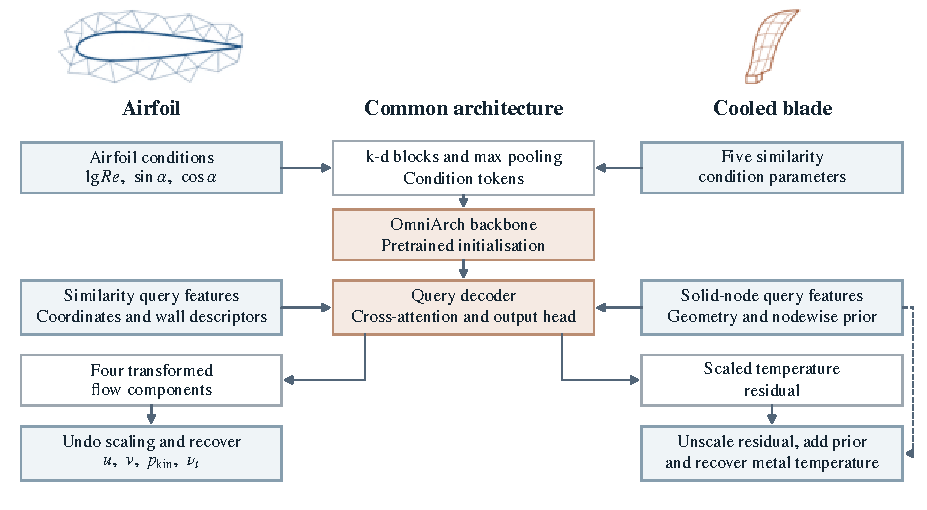
\includegraphics[width=.95\linewidth]{figs/fig2.pdf}
  \caption{Similarity transformations, common mesh encoding, and field reconstruction for the airfoil and blade tasks. The dashed path denotes reuse of the nodewise prior in the blade reconstruction. The two tasks use separately trained instances of the common architecture.}
  \label{fig:two-task-workflow}
\end{figure}

A k-d tree partitions each unstructured mesh into a fixed number of spatial blocks.
At each step, the block with the most nodes is split at the median along the coordinate
axis of greatest extent. The airfoil mesh uses $2048$ blocks and encodes all nodes
in each block. The blade solid mesh uses $4096$ blocks, with $32$ nodes sampled in each
block during preprocessing and reused across operating conditions.

The airfoil block features are the two spatial coordinates, the logarithm of the wall
distance, the two components of the wall normal, and a wall indicator. The normal
components are set to zero away from the wall. The blade features are the three
coordinates, radial distance from the rotation axis, and logarithmic distances to
the nearest fluid node and gas-side surface node. We append the standardised
temperature prior to these six geometry features at each blade query node.

A pointwise multilayer perceptron maps the node features before componentwise maximum
pooling within each block~\citep{Qi2017PointNet}. The pooled feature is mapped to a block token and combined
with a Fourier encoding of the block centre. We standardise airfoil conditions as in
Section~\ref{subsec:airfoil-similarity}. For the blade, each of the five condition
parameters is divided by its value in the $600\,\mathrm{K}$ case in $S_0$. Each scalar
is mapped to a condition token. The block tokens, condition tokens, and a trainable
summary token are passed to a backbone of width $1024$ with $16$ attention heads.
Its eight blocks and final normalisation are initialised from the first eight blocks
and final normalisation of OmniArch-base~\citep{Chen2025OmniArch}. The backbone and the new embedding,
decoding, and output modules are trained jointly for each task.

The decoder embeds the query features and uses one cross-attention layer~\citep{Vaswani2017} to read the
encoded block and condition tokens. Its output contains four standardised field
components for the airfoil or one scaled residual for the blade at each query.
Inference encodes each case once and reuses the encoded sequence across batches of
queries to recover the field at all target nodes.

Physics-informed neural networks incorporate governing-equation residuals into
the loss~\citep{Raissi2019}. Here, the similarity transformations and the temperature
prior define the supervised training targets. For $N_q$ query nodes and $C$ output components, let $y_{ic}$ and $\widehat y_{ic}$
denote the target and prediction for component $c$ at node $i$. With query weights
$w_i$ and component weights $a_c$, the weighted mean squared error is
\begin{equation}
  \label{eq:weighted-training-loss}
  \mathcal{L}=
  \frac{\displaystyle\sum_{i=1}^{N_q} w_i
    \left[\frac{1}{C}\sum_{c=1}^{C}a_c
      (\widehat y_{ic}-y_{ic})^2\right]}
       {\displaystyle\sum_{i=1}^{N_q}w_i}.
\end{equation}
The airfoil task uses $C=4$. Both airfoil configurations compute the loss in their
standardised output spaces. Each sample includes all wall nodes and up to $8000$
randomly selected off-wall nodes from one training case. The similarity configuration
sets the wall-node weight to $5$ and the pressure component weight to $2$. The
dimensional configuration uses unit weights and a seven-component query with the two
freestream velocity components and logarithmic wall distance. All remaining weights
are unity. Section~\ref{sec:airfrans-results} therefore compares the two full
configurations.

The blade task uses $C=1$ and the residual in Eq.~\eqref{eq:blade-training-residual}
divided by $\sigma_\theta$ as the target. Each sample includes $49152$ solid nodes from
one training condition, with $w_i=a_c=1$. Both tasks use AdamW~\citep{Loshchilov2019} with linear warmup and
cosine learning-rate decay. The airfoil runs use seeds $0$ to $2$ and are evaluated
separately. The blade runs use seeds $0$ to $4$. We average their predicted physical
temperatures nodewise before computing the ensemble error.
% Collect learning rates, training steps, hardware, and reproduction details in the appendix.

\section{Reynolds-number extrapolation on the AirfRANS benchmark}\label{sec:airfrans-results}
\noindent{\small\textbf{Page budget:} approx.\ 4 pages\quad \textbf{Status:} Draft ready for review}\par

\subsection{Benchmark splits and comparison setup}\label{subsec:airfrans-setup}
\noindent{\small\textbf{Page budget:} approx.\ 0.75 pages}\par

We evaluated the similarity and dimensional configurations on the same AirfRANS
Reynolds-number split. Both were trained on $504$ cases within the interval
$Re\in[3\times10^6,\,5\times10^6]$ and tested on $496$ cases outside it.
Fig.~\ref{fig:airfrans-operating-split} shows the $254$ test cases below the training
interval and the $242$ above it. Reynolds numbers were computed from the freestream
speeds in the official split manifest using the chord and viscosity specified in
Section~\ref{subsec:airfoil-similarity}. The airfoil geometry and freestream
conditions were provided for each case.

\begin{figure}[width=\linewidth,pos=htbp]
  \centering
  % Source: Dataset/manifest.json in the official AirfRANS Dataset.zip.
  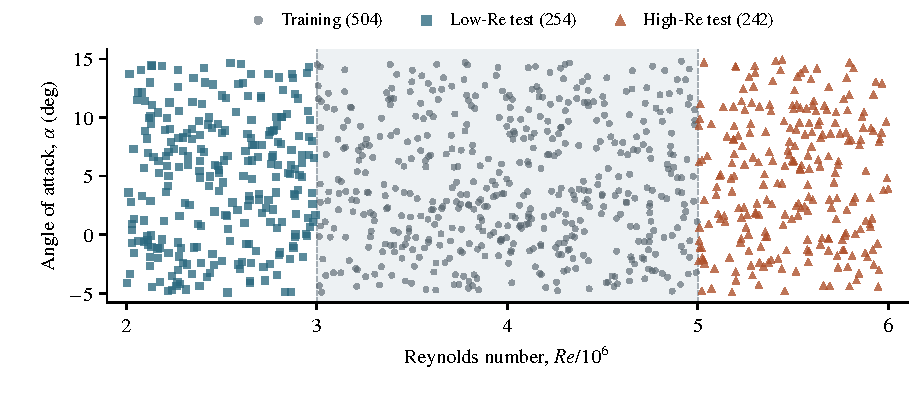
\includegraphics[width=.95\linewidth]{figs/fig3.pdf}
  \caption{AirfRANS case distribution in Reynolds number and angle of attack. Each point is one case in the official Reynolds-number split. The shaded band marks the training interval.}
  \label{fig:airfrans-operating-split}
\end{figure}

Both configurations used the same backbone initialisation and training schedule.
Table~\ref{tab:airfrans-configurations} summarises the differences in the
representations and loss weights described in Section~\ref{subsec:mesh-to-field}.

\begin{table}[width=.96\linewidth,cols=3,pos=htbp]
  \caption{Dimensional and similarity configurations used in the AirfRANS comparison.}
  \label{tab:airfrans-configurations}
  \begin{tabular*}{\tblwidth}{@{}LCC@{}}
    \toprule
    Setting & Dimensional configuration & Similarity configuration \\
    \midrule
    Condition vector & $(Re/10^6,\,\alpha/10,\,U_\infty/60)$
      & $(\lg Re,\,\sin\alpha,\,\cos\alpha)$ \\
    Query representation
      & \makecell[c]{Freestream velocity components\\and logarithmic wall distance}
      & \makecell[c]{Angle-of-attack features and\\Reynolds-scaled wall distances} \\
    Query dimension & $7$ & $8$ \\
    Field targets before standardisation
      & Dimensional fields & Similarity fields, Eq.~\eqref{eq:airfoil-forward} \\
    Wall-node weight & $1$ & $5$ \\
    Pressure-component weight & $1$ & $2$ \\
    \bottomrule
  \end{tabular*}
  \par\smallskip
  \begin{minipage}{\tblwidth}
    \footnotesize
    The dimensional condition vector uses the numerical angle of attack in degrees
    and freestream speed in \(\mathrm{m/s}\).
  \end{minipage}
\end{table}

We recovered the dimensional fields before applying the same AirfRANS aerodynamic
post-processing~\citep{Bonnet2022AirfRANS} to both configurations. For each of the three seeds ($0$, $1$, and
$2$), we computed a relative $L_2$ error of the lift coefficient over the full test set.
We report the mean and standard deviation of these three errors.
Spearman's rank correlation $\rho_L$ compares the ordering of the predicted and
reference lift coefficients across test cases.

\subsection{Lift prediction accuracy}\label{subsec:airfrans-errors}
\noindent{\small\textbf{Page budget:} approx.\ 2 pages}\par

Let $\Gamma_w$ denote the airfoil surface, $\mathbf{n}$ its unit normal pointing into
the fluid, and $\mathbf{s}_w$ the viscous traction per unit density for this normal
convention. The lift direction is $\mathbf{e}_L=(-\sin\alpha,\cos\alpha)$.
For unit span, the lift coefficient is
\begin{equation}
  \label{eq:airfrans-lift}
  C_L=\frac{2}{U_\infty^2 L}
      \int_{\Gamma_w}
      \left(-p_{\mathrm{kin}}\mathbf{n}+\mathbf{s}_w\right)
      \cdot\mathbf{e}_L\,\mathrm{d}\ell .
\end{equation}
The discrete integration uses surface segment lengths and point-to-cell averages
of the pressure, normal, and viscous traction. The chord is $L=1\,\mathrm{m}$.
For evaluation, we set the predicted wall velocity and turbulent kinematic viscosity
to zero, following the benchmark procedure. The traction term is computed from
the wall velocity gradient using the molecular viscosity. We applied the same
force calculation to the reference and predicted fields.

For a fixed geometry and operating condition, let $\delta$ denote the prediction
minus the reference. Subtracting the two lift integrals gives the error for one case.
To quantify the error over the test set, we form vectors $\widehat{\mathbf{C}}_L$
and $\mathbf{C}_L$ with one predicted and one reference coefficient per case. Thus,
\begin{equation}
  \label{eq:airfrans-lift-error}
  \begin{aligned}[b]
    &\delta C_L=\frac{2}{U_\infty^2 L}
      \int_{\Gamma_w}
        \left(-\delta p_{\mathrm{kin}}\mathbf{n}+\delta\mathbf{s}_w\right)
        \cdot\mathbf{e}_L\,\mathrm{d}\ell, \\
    &\varepsilon_{C_L}
      =\frac{\left\|\widehat{\mathbf{C}}_L-\mathbf{C}_L\right\|_2}
             {\left\|\mathbf{C}_L\right\|_2}.
  \end{aligned}
\end{equation}
The numerator combines the squared absolute coefficient errors across cases.
A single norm of the reference coefficients sets the scale for the test set.

The similarity configuration reduced the mean relative $L_2$ error of lift from
$0.0514$ to $0.0182$, a reduction of about $65\%$ on the shared test set
(Table~\ref{tab:airfrans-lift}). It also yielded a reported Spearman correlation
of $0.9996$, indicating close agreement with the reference lift ranking across
the $496$ cases. The relative error quantifies agreement in magnitude, and the
rank correlation quantifies agreement in ordering.

\begin{table}[width=.9\linewidth,cols=4,pos=htbp]
  \caption{Lift prediction accuracy on the 496 AirfRANS Reynolds-number extrapolation cases.}
  \label{tab:airfrans-lift}
  \begin{tabular*}{\tblwidth}{@{}LCCC@{}}
    \toprule
    Configuration & Seeds & Relative $L_2$ error of $C_L$ & Spearman $\rho_L$ \\
    \midrule
    Dimensional & $3$ & $0.0514\pm0.0038$ & \textemdash \\
    Similarity & $3$ & $0.0182\pm0.0026$ & $0.9996$ \\
    \bottomrule
  \end{tabular*}
  \par\smallskip
  \begin{minipage}{\tblwidth}
    \footnotesize
    Each configuration was trained on $504$ cases. The relative $L_2$ error is defined
    in Eq.~\eqref{eq:airfrans-lift-error} and reported as the mean $\pm$ standard deviation
    across seeds $0$, $1$, and $2$. The single $\rho_L$ value is taken from the
    experiment summary. The dash marks an unavailable rank correlation.
  \end{minipage}
\end{table}

Fig.~\ref{fig:airfrans-lift-parity} is reserved for the casewise comparison behind
the aggregate errors in Table~\ref{tab:airfrans-lift}. The planned panels use
common axes for both configurations and distinguish the two extrapolation ranges.

\begin{figure}[width=\linewidth,pos=htbp]
  \centering
  \figureguide{Casewise lift comparison (figure pending)}
    {Paired reference and predicted $C_L$ from the per-case \texttt{metrics.json} for
     both configurations and seeds 0, 1 and 2. Join to the Reynolds split by case ID.}
    {Use one panel per configuration, with reference $C_L$ on the horizontal axis and
     predicted $C_L$ on the vertical axis. Use common limits, equal axis scales and an
     identity line. Distinguish low- and high-$Re$ cases by marker.}
    {Each panel must contain 496 pairs per seed (254 low-$Re$, 242 high-$Re$).
     Recompute Eq.~\eqref{eq:airfrans-lift-error} per seed and match the rounded
     mean and standard deviation in Table~\ref{tab:airfrans-lift}.}
  \fbox{\parbox[c][42mm][c]{.88\linewidth}{\centering\strut}}
  \caption{Planned comparison of predicted and reference lift coefficients in the two extrapolation ranges.}
  \label{fig:airfrans-lift-parity}
\end{figure}

The pressure contribution in Eq.~\eqref{eq:airfrans-lift-error} depends on both the
local pressure error and the surface normal. Pressure discrepancies on different
parts of the surface can reinforce or cancel one another in the lift integral.
A small lift error can therefore coexist with local pressure errors.
Fig.~\ref{fig:airfrans-pressure-fields} is reserved for a spatial comparison pairing
the pressure fields with surface pressure-coefficient profiles. The selection rule
uses one case from each side of the training interval, choosing the case closest
to the median Reynolds number on that side.

\begin{figure}[width=\linewidth,pos=htbp]
  \centering
  \figureguide{Pressure fields and surface profiles (figure pending)}
    {AirfRANS reference meshes and nodal pressures, matched model pressure predictions,
     surface coordinates, freestream speed and the lift error for each selected case.}
    {Use one row per $Re$ range. Select the case nearest its range median, breaking
     ties by case ID. Plot reference and predicted $p_{\rm kin}$ on a shared scale,
     signed error on a scale centred at zero, and upper- and lower-surface $C_p$ against $x/L$.}
    {Give case ID, $Re$, angle of attack, configuration, seed and lift error for each row.
     On matched nodes check that the error is prediction minus reference and that
     $C_p=2p_{\rm kin}/U_\infty^2$ for both profiles.}
  \fbox{\parbox[c][62mm][c]{.88\linewidth}{\centering\strut}}
  \caption{Planned pressure-field and surface-pressure comparisons for representative low- and high-Reynolds-number cases.}
  \label{fig:airfrans-pressure-fields}
\end{figure}

\subsection{Analysis of extrapolation performance and inference time}\label{subsec:airfrans-comparison}
\noindent{\small\textbf{Page budget:} approx.\ 1.25 pages}\par

The improvement in Table~\ref{tab:airfrans-lift} compares the two configurations in
Table~\ref{tab:airfrans-configurations}. Field representation, query features,
and loss weighting changed together. Evaluation of the original
checkpoints with the current implementation reproduced the reported mean and
standard deviation for each configuration.

We tested the influence of the encoded geometry by substituting the spatial block
tokens of another airfoil. The measured output change was about $0.24$ on a
reported normalised output scale of $0.72$. This response shows that the airfoil
predictions were sensitive to the geometric information supplied through the block
tokens. Section~\ref{subsec:blade-discussion} examines the corresponding behaviour
for the blade task, where all operating conditions share one mesh.

The experiment summary reports a flow prediction time of approximately
$0.22\,\mathrm{s}$ per case and a RANS computation time of about $25\,\mathrm{min}$.
In the current implementation, the timer brackets one prediction call for one
checkpoint with GPU synchronisation. This interval includes loading the prepared case,
encoding and decoding the field, and returning the dimensional predictions to the host.
The timing window ends before output files are written and aerodynamic coefficients
are evaluated.
% Confirm the hardware, mesh size, and timing boundaries for both reported values
% against the original timing records before using them for a speedup comparison.

\section{Temperature extrapolation for a cooled turbine blade}\label{sec:blade-results}
\noindent{\small\textbf{Page budget:} approx.\ 4 pages\quad \textbf{Status:} Draft ready for review}\par

\subsection{Blade case and baseline methods}\label{subsec:blade-setup}
\noindent{\small\textbf{Page budget:} approx.\ 1 page}\par
% Verify the material properties and complete boundary conditions against the original CFX project.

The blade study used seven converged CFX conjugate heat transfer solutions on the same
cooled rotor blade. Each temperature field was evaluated on the common mesh of
$3{,}304{,}055$ solid nodes. The gas-side surface was extracted from the CFX region
\emph{surface Shadow} and contained $95{,}837$ solid nodes. In all seven cases, the reconstructed
surface reproduced the CFX area-weighted mean temperature of that region to within
$3\times10^{-5}\,\mathrm{K}$. The extracted node coordinates were identical across
the cases, providing the correspondence used by the nodewise prior.

Table~\ref{tab:blade-cases} identifies the five training cases, the three training cases
used to fit the prior, and the two high-temperature test cases. Both test cases used
the same three low-temperature solutions to construct their priors. The two training
cases at $T_g=600\,\mathrm{K}$ had different coolant inlet total temperatures, and
only the designated prior case contributed to the fit.

\begin{table}[width=.92\linewidth,cols=6,pos=htbp]
  \caption{Inlet total temperatures and roles of the seven cooled-blade cases.}
  \label{tab:blade-cases}
  \begin{tabular*}{\tblwidth}{@{}LCCCCC@{}}
    \toprule
    Case ID & $T_g$ (K) & $T_c$ (K) & Training & Prior fit & Test \\
    \midrule
    e3-model-600K\_001  &  600.0 & 334.5 & Yes & Yes & \textemdash \\
    e3-model-800K\_001  &  800.0 & 445.0 & Yes & Yes & \textemdash \\
    e3-model-1000K\_001 & 1000.0 & 557.5 & Yes & Yes & \textemdash \\
    e3-unmodel-600K\_001 & 600.0 & 401.4 & Yes & \textemdash & \textemdash \\
    e3\_redown40\_001   &  683.8 & 344.0 & Yes & \textemdash & \textemdash \\
    e3-model-1200K\_001 & 1200.0 & 669.0 & \textemdash & \textemdash & Yes \\
    e3-1616K\_001       & 1616.0 & 901.0 & \textemdash & \textemdash & Yes \\
    \bottomrule
  \end{tabular*}
\end{table}

The three prior-fit cases and both tests have
\(T_c/T_g\) between \(0.556\) and \(0.558\). The tests extend \(T_g\) beyond
the highest training temperature of \(1000\,\mathrm{K}\) at a similar inlet
temperature ratio. The two auxiliary training cases cover other ratios.

We compared three temperature reconstructions on this mesh. The direct similarity
baseline transferred the dimensionless field from the prior case closest in $T_g$.
For both tests, this was the $1000\,\mathrm{K}$ case. The linear-prior baseline
evaluated Eq.~\eqref{eq:blade-linear-prior} at the target $T_g$. The full model
added the learned residual to that prior. Each method then used the target $T_g$
and $T_c$ to recover the metal temperature through
Eq.~\eqref{eq:blade-temperature-similarity}.

\subsection{Solid-domain temperature prediction error}\label{subsec:blade-errors}
\noindent{\small\textbf{Page budget:} approx.\ 1.75 pages}\par

For the full model, we averaged the temperatures from the five training seeds
($0$ to $4$) at each solid node before computing the error against CFX. Let
$\widehat T_i^{(m)}$ be the temperature predicted at node $i$ by model $m$,
$T_i$ the CFX reference temperature, and $N_s$ the number of solid nodes. For
$M=5$, the ensemble prediction and its mean absolute error (MAE) are
\begin{equation}
  \label{eq:blade-ensemble-mae}
  \begin{aligned}[b]
    &\widehat T_i^{\,\mathrm{ens}}
      =\frac{1}{M}\sum_{m=1}^{M}\widehat T_i^{(m)}, \\
    &\mathrm{MAE}_T^{\,\mathrm{ens}}
      =\frac{1}{N_s}\sum_{i=1}^{N_s}
       \left|\widehat T_i^{\,\mathrm{ens}}-T_i\right|.
  \end{aligned}
\end{equation}
The MAE weights the solid nodes equally and is computed for each test condition
separately.

The full model achieved the lowest solid-node MAE at both test conditions
(Table~\ref{tab:blade-temperature-mae}). At $T_g=1200\,\mathrm{K}$, the MAE decreased
from $5.32\,\mathrm{K}$ with direct similarity conversion to $1.84\,\mathrm{K}$ with
the linear prior and $1.56\,\mathrm{K}$ with the residual correction. At
$T_g=1616\,\mathrm{K}$, the corresponding errors were $20.96$, $5.34$, and
$4.90\,\mathrm{K}$. For the latter condition, $T_c=901\,\mathrm{K}$, so
Eq.~\eqref{eq:blade-temperature-error} gives the equivalent dimensionless MAE
$4.90/715\approx0.00685$ for the ensemble.

\begin{table}[width=.9\linewidth,cols=3,pos=htbp]
  \caption{Metal-temperature prediction error at the two out-of-range blade conditions.}
  \label{tab:blade-temperature-mae}
  \begin{tabular*}{\tblwidth}{@{}LCC@{}}
    \toprule
    \multirow[c]{2}{*}[-\dimexpr(\aboverulesep+\belowrulesep+\cmidrulewidth)/2\relax]{Method}
    & \multicolumn{2}{c}{Solid-node MAE (K)} \\
    \cmidrule(l){2-3}
    & $T_g=1200\,\mathrm{K}$ & $T_g=1616\,\mathrm{K}$ \\
    \midrule
    Direct similarity conversion & $5.32$ & $20.96$ \\
    Nodewise linear temperature prior & $1.84$ & $5.34$ \\
    Prior with learned residual & $1.56$ & $4.90$ \\
    \bottomrule
  \end{tabular*}
  \par\smallskip
  \begin{minipage}{\tblwidth}
    \footnotesize
    Each MAE weights all solid nodes equally. The baseline fields were evaluated
    directly. The final row uses the nodewise ensemble in Eq.~\eqref{eq:blade-ensemble-mae}.
  \end{minipage}
\end{table}

The solid-domain MAE describes average error across the mesh. Local thermal
assessment also depends on the magnitude and position of the hottest regions.
We distinguish the peak-temperature error $\max_i \widehat T_i-\max_i T_i$
from the temperature error at the reference hotspot. The hotspot displacement is
the Euclidean distance between the predicted and reference maximum-temperature
nodes. The gas-side surface MAE assesses the subset of nodes on that interface.
Table~\ref{tab:blade-local-errors} reserves the local-error comparison, and
Fig.~\ref{fig:blade-temperature-fields} reserves the corresponding fields.
% Populate the gas-side MAE, peak-temperature error, and hotspot displacement from
% the per-case evaluation output when the reference and predicted fields are available.

\begin{table}[width=.96\linewidth,cols=5,pos=htbp]
  \displayguide{\tblwidth}{Local temperature and hotspot errors (table pending)}
    {Per-case blade \texttt{metrics.json} for both tests and all three methods.
     Dashes mark values awaiting evaluation.}
    {Use the direct-conversion, linear-prior and five-seed mean-field results.
     Fill the three columns from \texttt{outer\_mae\_K}, \texttt{Tmax\_err\_K}
     and \texttt{hotspot\_dist\_mm}, respectively.}
    {Check all 18 entries by case and method. Gas-side MAE averages absolute errors
     over surface nodes (K). Peak bias is $\max\widehat T-\max T$ (K).
     Hotspot shift is the distance between the two peak nodes (mm).}
  \caption{Local metal-temperature and hotspot errors at the two blade test conditions.}
  \label{tab:blade-local-errors}
  \begin{tabular*}{\tblwidth}{@{}LLCCC@{}}
    \toprule
    $T_g$ (K) & Method & Gas-side MAE (K) & Peak bias (K) & Hotspot shift (mm) \\
    \midrule
    \multirow[c]{3}{*}{1200}
      & Direct similarity & \textemdash & \textemdash & \textemdash \\
      & Nodewise linear prior & \textemdash & \textemdash & \textemdash \\
      & Prior with learned residual & \textemdash & \textemdash & \textemdash \\
    \midrule
    \multirow[c]{3}{*}{1616}
      & Direct similarity & \textemdash & \textemdash & \textemdash \\
      & Nodewise linear prior & \textemdash & \textemdash & \textemdash \\
      & Prior with learned residual & \textemdash & \textemdash & \textemdash \\
    \bottomrule
  \end{tabular*}
\end{table}

\begin{figure}[width=\linewidth,pos=htbp]
  \centering
  \figureguide{Blade temperature fields and hotspots (figure pending)}
    {Solid-node coordinates and gas-side surface mesh, CFX nodal temperatures, and
     matching five-seed mean temperature fields for the 1200 and 1616\,K cases.}
    {Use one row per case. Show CFX temperature, ensemble temperature and absolute
     error (K) from the same viewpoint. Share the temperature scale within each row.
     Label the gas-side surface and section shown. Locate both peak nodes on the blade.}
    {Compute $|\widehat T^{\rm ens}-T|$ after averaging the five predictions at each node.
     Its all-node mean must round to 1.56\,K at 1200\,K and 4.90\,K at 1616\,K.
     Check the marked peak separation against Table~\ref{tab:blade-local-errors}.}
  \fbox{\parbox[c][62mm][c]{.88\linewidth}{\centering\strut}}
  \caption{Planned comparison of the reference and ensemble temperature fields, absolute errors and hotspot locations.}
  \label{fig:blade-temperature-fields}
\end{figure}

\subsection{Contribution and scope of the temperature prior}\label{subsec:blade-discussion}
\noindent{\small\textbf{Page budget:} approx.\ 1.25 pages}\par\nopagebreak[4]

The nodewise prior accounted for most of the observed reduction in MAE relative
to direct similarity conversion. At $1616\,\mathrm{K}$, it reduced the MAE by
$15.62\,\mathrm{K}$, and the learned residual reduced it by a further
$0.44\,\mathrm{K}$. The corresponding reductions at $1200\,\mathrm{K}$ were
$3.48\,\mathrm{K}$ and $0.28\,\mathrm{K}$.

Input perturbations on the original blade checkpoints probed the sensitivity of
the residual prediction to the encoded inputs. Replacing the spatial block tokens by noise,
setting them to zero, or halving the five global condition parameters changed the
output by less than $10^{-8}$ on an output scale of approximately $10^{-3}$.
The nodewise prior remained in the query during these tests. All blade cases share
the same mesh, and the prior already supplies case-dependent information at each
location. The small responses support interpreting the trained blade network as
a nodewise correction to the prior on this geometry. In the airfoil task
(Section~\ref{subsec:airfrans-comparison}), substituting the tokens from a different
geometry produced a measurable response on the airfoil output scale
(Fig.~\ref{fig:encoder-diagnostics}).

\begin{figure}[width=\linewidth,pos=htbp]
  \centering
  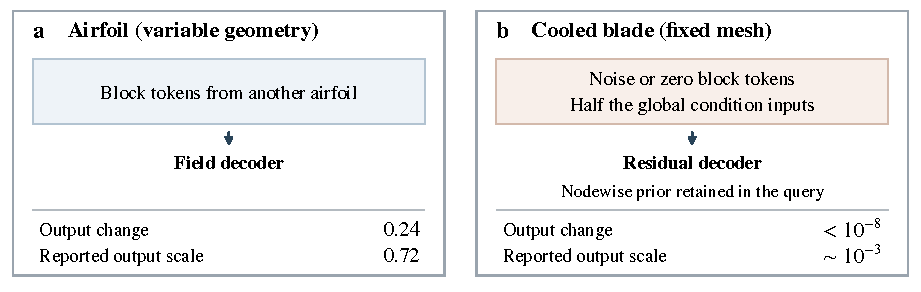
\includegraphics[width=.95\linewidth]{figs/fig7.pdf}
  \caption{Responses to input perturbations in the airfoil and cooled-blade tasks. Each panel reports the output change against that model's own output scale. The blade query retained the nodewise temperature prior during the perturbations.}
  \label{fig:encoder-diagnostics}
\end{figure}

The inlet temperature difference in Eq.~\eqref{eq:blade-temperature-similarity}
sets the scale for converting the dimensionless field back to kelvin. The
normalised temperature can still change when the operating condition changes
the effective thermal properties and interfacial heat transfer~\citep{Cartlidge2024}. The test results
establish the benefit of fitting this variation on the fixed rotor blade. Applying
the nodewise procedure to a different blade or mesh requires a correspondence
between solid nodes or a prior fitted on the new mesh.

\section{Conclusion}\label{sec:conclusion}
\noindent{\small\textbf{Page budget:} approx.\ 1 page\quad \textbf{Status:} Draft ready for review}\par

OmniArch-Aero incorporates task-specific similarity representations into field
prediction on unstructured meshes at operating conditions beyond the training
range. The airfoil model predicts flow fields in similarity variables for
Reynolds-number extrapolation. The blade model reconstructs metal temperatures
at higher inlet temperatures by combining a nodewise temperature prior with
a learned residual. The two tasks use the same mesh-to-field architecture and
are trained separately.

On the same $496$ AirfRANS extrapolation cases, the lift-coefficient relative
$L_2$ error decreased from \mbox{$0.0514\pm0.0038$} for the dimensional configuration
to \mbox{$0.0182\pm0.0026$} for the similarity configuration (mean $\pm$ standard
deviation over three runs, Table~\ref{tab:airfrans-lift}). For the cooled
blade at $T_g=1616\,\mathrm{K}$, the solid-node mean absolute error was
$20.96\,\mathrm{K}$ with direct similarity conversion, $5.34\,\mathrm{K}$
with the linear prior, and $4.90\,\mathrm{K}$ with the five-model ensemble
that included learned residuals (Table~\ref{tab:blade-temperature-mae}).

The airfoil token substitution test showed that the prediction was sensitive
to the encoded geometry. On the fixed blade mesh, the prior accounted for
most of the observed error reduction, and the perturbation tests support
interpreting the network as a nodewise correction to that prior. Extending
this procedure to a different blade or mesh requires a node correspondence
or a prior fitted on the new mesh. Tests across multiple blade geometries
could determine when geometric encoding improves temperature prediction.

% To print the credit authorship contribution details
\printcredits

\appendix

\bibliographystyle{cmame-num}
\bibliography{cas-refs}

% Biography
%\bio{}
% Here goes the biography details.
%\endbio

%\bio{pic1}
% Here goes the biography details.
%\endbio

\end{document}

